\documentclass[a4paper, 11pt]{article}
\usepackage{geometry}
\usepackage{url}
\usepackage{color}
\usepackage{graphicx}
\linespread{1}
\geometry{a4paper,top=3cm,left=3cm,right=2.5cm,bottom=2cm}
\usepackage{hyperref}
\hypersetup{colorlinks,linkcolor=black,citecolor=blue}
\title{\textbf{Laboratory assignment} \\[1ex] \large \textbf{Component 3: Conceptual Analysis and Design}}
\author{\textbf{Authors: Ichim Stefan, Mirt Leonard} \\ \textbf{Group: 246/1}}
\begin{document}
\maketitle

\section{Conceptual Modeling Using Agents (PAGES)}

\subsection{Pac-Man System Overview}
The Pac-Man game simulation is conceptually modeled as a multi-agent system using the PAGES framework (Perception, Action, Goal, Environment, State). This approach provides a systematic way to analyze the agents and their interactions within the system.

\subsection{PAGES Model Components}

\begin{table}[h]
\centering
\caption{PAGES Model for Pac-Man Agent}
\begin{tabular}{|p{2.5cm}|p{11cm}|}
\hline
\textbf{Perception (P)} & 
\begin{itemize}
    \item Local maze visibility (walls, dots, power pellets)
    \item Ghost positions and states within perception radius
    \item Score changes and remaining lives
\end{itemize} \\
\hline
\textbf{Actions (A)} & 
\begin{itemize}
    \item Movement in four directions (UP, DOWN, LEFT, RIGHT)
    \item Collection of dots and power pellets
    \item Consumption of vulnerable ghosts
\end{itemize} \\
\hline
\textbf{Goals (G)} & 
\begin{itemize}
    \item Maximize score by collecting all dots and power pellets
    \item Avoid ghosts in normal state
    \item Consume ghosts when vulnerable
\end{itemize} \\
\hline
\textbf{Environment (E)} & Grid-based maze with walls, dots, power pellets, and tunnels \\
\hline
\textbf{State (S)} & Position, direction, and power status (normal or powered-up) \\
\hline
\end{tabular}
\end{table}

\begin{table}[h]
\centering
\caption{PAGES Model for Ghost Agents}
\begin{tabular}{|p{2.5cm}|p{11cm}|}
\hline
\textbf{Perception (P)} & 
\begin{itemize}
    \item Local maze visibility
    \item Pac-Man's position (when within perception radius)
    \item Current behavior mode (chase, scatter, frightened)
\end{itemize} \\
\hline
\textbf{Actions (A)} & 
\begin{itemize}
    \item Movement in four directions
    \item Return to ghost house when consumed
    \item Respawn from ghost house
\end{itemize} \\
\hline
\textbf{Goals (G)} & 
\begin{itemize}
    \item Blinky: Direct pursuit of Pac-Man
    \item Pinky: Intercept Pac-Man ahead of his path
    \item Inky: Flank Pac-Man through coordination
    \item Clyde: Alternate between pursuit and patrol
\end{itemize} \\
\hline
\textbf{Environment (E)} & Same grid-based maze as Pac-Man with ghost house region \\
\hline
\textbf{State (S)} & Position, direction, and mode (normal, frightened, returning) \\
\hline
\end{tabular}
\end{table}

\clearpage

\begin{table}[h]
\centering
\caption{PAGES Model for Environment Agent}
\begin{tabular}{|p{2.5cm}|p{11cm}|}
\hline
\textbf{Perception (P)} & 
\begin{itemize}
    \item Complete maze state
    \item All agent positions and states
    \item Game timer and score information
\end{itemize} \\
\hline
\textbf{Actions (A)} & 
\begin{itemize}
    \item Update maze state
    \item Signal mode changes to ghosts
    \item Process collisions between agents
    \item Progress game level and visualization
\end{itemize} \\
\hline
\textbf{Goals (G)} & 
\begin{itemize}
    \item Maintain game consistency
    \item Enforce rules and fair progression
    \item Provide visualization and scoring
\end{itemize} \\
\hline
\textbf{Environment (E)} & The entire game system it manages and coordinates \\
\hline
\textbf{State (S)} & Complete game state including all agents, maze elements, and timers \\
\hline
\end{tabular}
\end{table}

\section{Properties of the Environment}

The Pac-Man environment can be characterized according to standard properties of multi-agent environments. The table below summarizes these key properties:

\begin{table}[h]
\centering
\caption{Properties of the Pac-Man Environment}
\begin{tabular}{|p{4cm}|p{3cm}|p{7cm}|}
\hline
\textbf{Property} & \textbf{Classification} & \textbf{Key Characteristics} \\
\hline
Accessibility & Partially Accessible & 
\begin{itemize}
    \item Environment Agent: complete accessibility
    \item Pac-Man/Ghosts: limited by perception radius
\end{itemize} \\
\hline
Determinism & Deterministic & 
\begin{itemize}
    \item Predictable outcomes for actions
    \item Well-defined transition function
\end{itemize} \\
\hline
Episodic vs Sequential & Sequential & 
\begin{itemize}
    \item Current decisions affect future states
    \item Power pellet timing creates dependencies
\end{itemize} \\
\hline
Static vs Dynamic & Dynamic & 
\begin{itemize}
    \item Game state evolves independently
    \item Timer-based mode changes occur
\end{itemize} \\
\hline
Discrete vs Continuous & Discrete & 
\begin{itemize}
    \item Grid-based positions
    \item Discrete time steps and actions
\end{itemize} \\
\hline
Agent Structure & Multi-agent & 
\begin{itemize}
    \item Multiple concurrent agents
    \item Mix of cooperation and competition
\end{itemize} \\
\hline
State Dependency & Primarily Markovian & 
\begin{itemize}
    \item Next state depends on current state and actions
    \item Limited non-Markovian elements in ghost behavior
\end{itemize} \\
\hline
\end{tabular}
\end{table}

\clearpage

\section{Design of the Application}

\subsection{Class Diagram}
The Pac-Man multi-agent system is built around several core object classes that define the structure and behavior of the simulation. The following class diagrams illustrate the main components of the system.

\subsubsection{Agent Classes}
The agent hierarchy consists of a base Agent class extended by PacManAgent and GhostAgent classes. The GhostAgent is further specialized into four distinct ghost types, each with unique targeting and behavior patterns.

\begin{figure}[h]
\centering
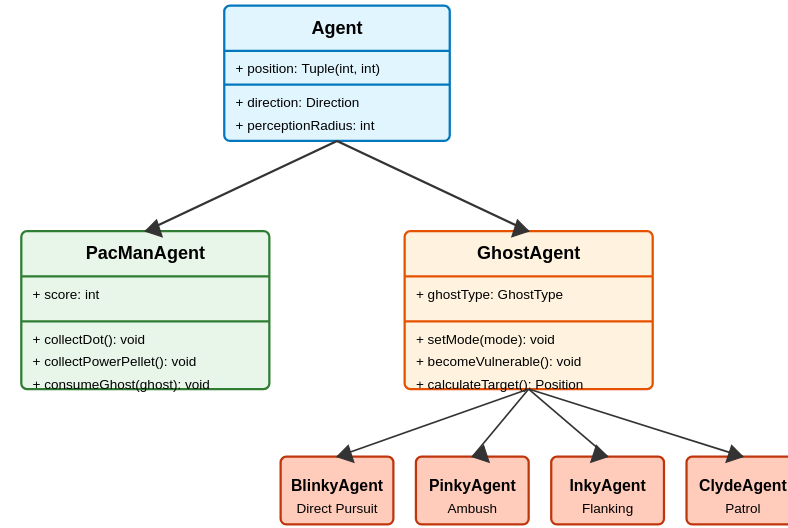
\includegraphics[width=0.95\textwidth]{agent-class-diagram.png}
\caption{Pac-Man and Ghost Agent Class Hierarchy}
\end{figure}

Key features of the agent classes:
\begin{itemize}
    \item \textbf{Agent}: Abstract base class defining common properties such as position, direction, and perception radius
    \item \textbf{PacManAgent}: Implements dot collection, power pellet effects, and ghost consumption
    \item \textbf{GhostAgent}: Defines common ghost behaviors including mode changes and vulnerability states
    \item \textbf{Specialized Ghosts}: Each ghost type implements unique targeting strategies:
    \begin{itemize}
        \item Blinky: Direct pursuit targeting Pac-Man's current position
        \item Pinky: Ambush tactics targeting positions ahead of Pac-Man
        \item Inky: Flanking behavior using both Blinky and Pac-Man positions
        \item Clyde: Alternating between pursuit and patrol behaviors
    \end{itemize}
\end{itemize}

\subsubsection{Environment System}
The environment system consists of three main components: the EnvironmentAgent that manages the game state, the Maze that defines the playfield, and the Blackboard that facilitates agent communication.

\begin{figure}[h]
\centering
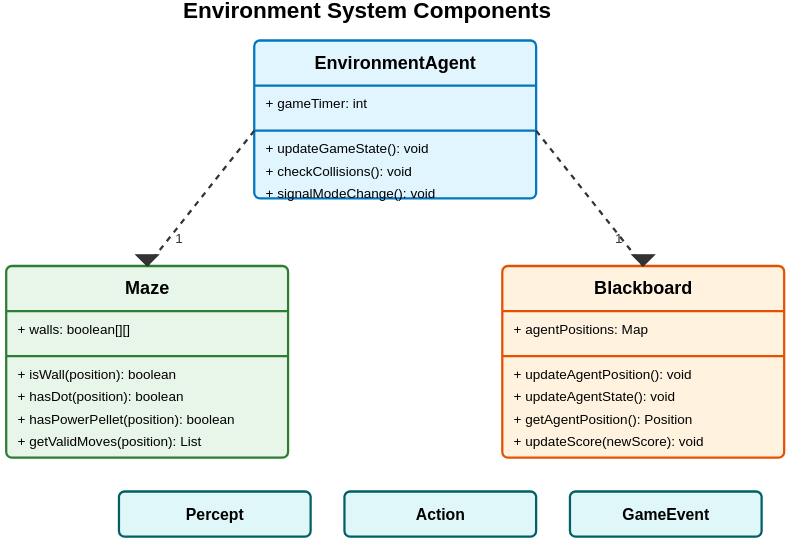
\includegraphics[width=0.95\textwidth]{environment-class-diagram.png}
\caption{Environment System Components}
\end{figure}

Key components of the environment system:
\begin{itemize}
    \item \textbf{EnvironmentAgent}: Coordinates the game simulation, manages collisions, and controls ghost mode transitions
    \item \textbf{Maze}: Represents the physical game space with walls, dots, power pellets, and provides navigation utilities
    \item \textbf{Blackboard}: Serves as the central knowledge repository, storing agent positions, game state, and facilitating indirect communication
    \item \textbf{Support Classes}: Include Percept, Action, and GameEvent structures that facilitate agent interaction
\end{itemize}

This modular design enables clean separation of concerns while providing the necessary communication channels between components. The agent-based architecture allows for autonomous decision-making while the environment system maintains game consistency and rule enforcement.

\section{Communication and Interaction Model}

\subsection{Communication Architecture}
The Pac-Man multi-agent system employs a hybrid communication architecture that balances efficiency with flexibility.

\begin{table}[h]
\centering
\caption{Communication Mechanisms in Pac-Man MAS}
\begin{tabular}{|p{3.5cm}|p{10.5cm}|}
\hline
\textbf{Mechanism} & \textbf{Purpose and Characteristics} \\
\hline
Blackboard Pattern & 
\begin{itemize}
    \item Central knowledge repository for shared game state
    \item Asynchronous, non-direct communication
    \item Suitable for non-time-critical information
\end{itemize} \\
\hline
Direct Messaging & 
\begin{itemize}
    \item Point-to-point agent communication
    \item Used for time-critical interactions
    \item Event-driven notifications
\end{itemize} \\
\hline
\end{tabular}
\end{table}

\subsection{Blackboard Structure and Access}

\begin{table}[h]
\centering
\caption{Blackboard Access Patterns}
\begin{tabular}{|p{3cm}|p{5.5cm}|p{5.5cm}|}
\hline
\textbf{Agent} & \textbf{Read Access} & \textbf{Write Access} \\
\hline
Environment Agent & Complete game state & All sections \\
\hline
Pac-Man Agent & Ghost positions and modes & Own position, dot collection events \\
\hline
Ghost Agents & Pac-Man position, other ghosts & Own position and mode \\
\hline
\end{tabular}
\end{table}

\subsection{Message Types}

The following message types facilitate direct communication between agents:

\begin{itemize}
    \item \textbf{ModeChangeMessage}: Notifies ghosts of behavior mode transitions
    \item \textbf{CollisionMessage}: Communicates agent interaction outcomes
    \item \textbf{StateTransitionMessage}: Signals significant game state changes
\end{itemize}

\clearpage

\subsection{Core Interaction Protocols}

\begin{table}[h]
\centering
\caption{Key Interaction Protocols}
\begin{tabular}{|p{3.5cm}|p{10.5cm}|}
\hline
\textbf{Protocol} & \textbf{Key Steps} \\
\hline
Game Cycle & 
\begin{enumerate}
    \item Update timers and check transitions
    \item Agents perceive environment
    \item Agents decide and execute actions (prioritized)
    \item Resolve interactions and update state
    \item Generate visualization
\end{enumerate} \\
\hline
Collision Resolution & 
\begin{enumerate}
    \item Detect position coincidence
    \item Check ghost vulnerability status
    \item Execute appropriate outcome (score update or life loss)
    \item Update agent positions and states
\end{enumerate} \\
\hline
Power Pellet Effect & 
\begin{enumerate}
    \item Pac-Man collects power pellet
    \item Notify all ghosts of frightened mode
    \item Start timer and track duration
    \item Restore normal ghost behavior when expired
\end{enumerate} \\
\hline
\end{tabular}
\end{table}

% \cite{Weiss1999}
% \cite{Russell1995}
%
% \bibliographystyle{alpha}
% \bibliography{biblio}
\end{document}
